\section{Methodology} \label{sec:methods}

The images used in this study underwent standard reduction techniques, including overscan, bias, dark, and defects reduction. Defects reduction involves creating maps that indicate regions with both bright and dark defects, such as dead pixels. These reductions serve as the starting state for the PTC study. Subsequently, other corrections, such as linearity and crosstalk, are applied to analyze their effects on the main parameters of the camera.

\vspace{3mm}
Professor Craig Lage generated supercalibrations for the entire focal plane, which are stored in his personal collection at \textit{u/cslage/calib/13144/calib.20220103}. The images shown in Figures \ref{fig:superbias} and \ref{fig:superdark} are superbias and superdarks, respectively, generated as part of the learning process for producing the calibration images using the LSST's software called \textit{DM stack}.

\vspace{3mm}
The code used to generate the calibration images via \textit{DM stack} can be found at \\ \href{https://github.com/lsst/cp_pipe}{https://github.com/lsst/cp\_pipe}. This code generates the data for the construction of the PTC and calculates the gain for each CCD segment as its FWC. Additionally, it calculates the gain using another method, which was analyzed in Section \ref{subsec:method_gainflat} to determine the differences between it and the PTC method. The alternative method involves using two pairs of flats for gain estimation. We utilized two versions of the \textit{DM stack} code\footnote{The DM stack software is developed for the LSST and is publicly available on GitHub at \href{https://github.com/lsst/}{https://github.com/lsst/}} for the entire focal plane:

\begin{itemize}
    \item w\_2022\_27: Initial version we started working with.
    \item w\_20222\_32: Version that includes one of our main results on obtaining the gain with pairs of flats (see the \href{https://jira.lsstcorp.org/browse/DM-35790}{DM-35790} ticket in Jira).
\end{itemize}

BPS (Batch Processing Service) was utilized to run the two previous versions. Detailed instructions on how to build the configuration files, handle possible errors, and access more information can be found in the GitHub repository of this project, \href{https://github.com/linagiraldom/RECA_Internship_Project}{RECA\_Internship\_Project}, in the notebook \href{https://github.com/linagiraldom/RECA_Internship_Project/blob/main/Notebooks/BPS_LSST.ipynb}{BPS\_LSST.ipynb}. Additionally, all the notebooks used to carry out the methodology described below are available in this repository. There is also a tutorial notebook called \href{https://github.com/linagiraldom/RECA_Internship_Project/blob/main/Notebooks/Tutorial.ipynb}{Tutorial.ipynb}, where I provide an overview of the \textit{Data Butler}, the API that manages and stores the data. It includes information on collections, image visualization, data retrieval, and other details related to the calibration images.

\begin{figure}[!htb]
     \centering
     \begin{subfigure}[b]{0.49\textwidth}
         \centering
         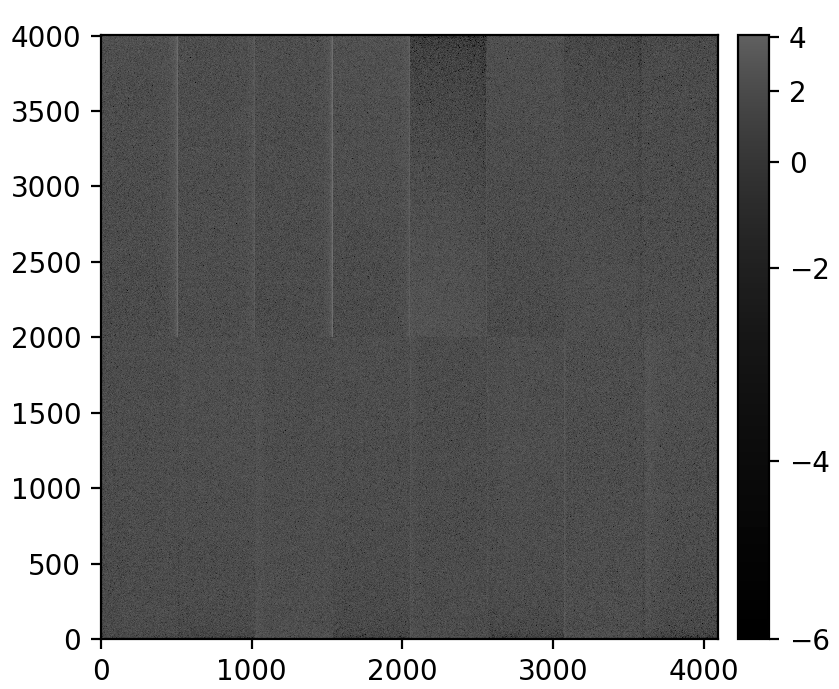
\includegraphics[width=\textwidth]{Figures/Super_bias_55.png}
     \end{subfigure}
     \hfill
     \begin{subfigure}[b]{0.49\textwidth}
         \centering
         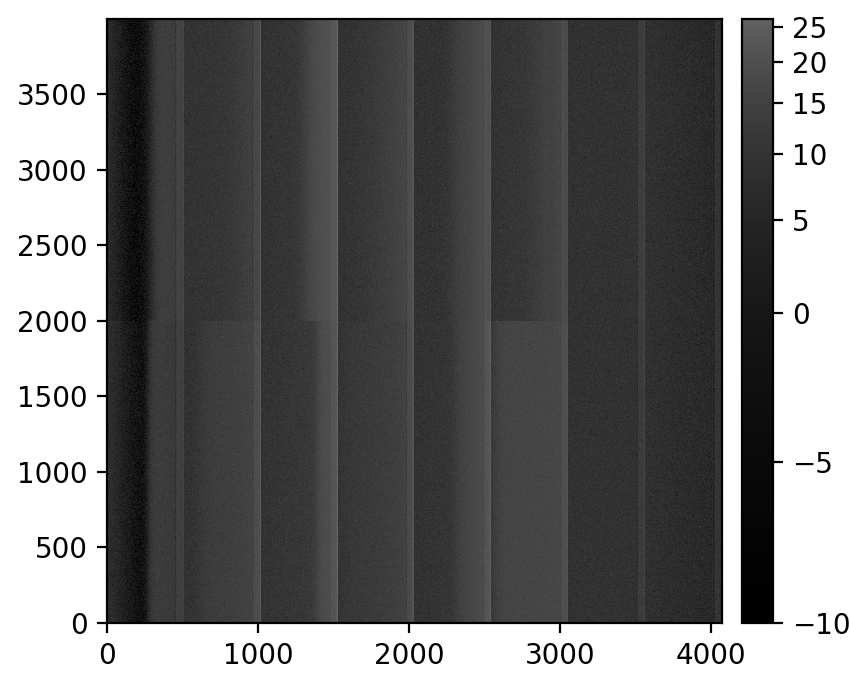
\includegraphics[width=\textwidth]{Figures/Super_bias_74.png}
     \end{subfigure}
        \caption{Masterbias images for detectors 55 (E2V) on the left and 74 (ITL) on the right.}
        \label{fig:superbias}
\end{figure}

\begin{figure}[!htb]
     \centering
     \begin{subfigure}[b]{0.49\textwidth}
         \centering
         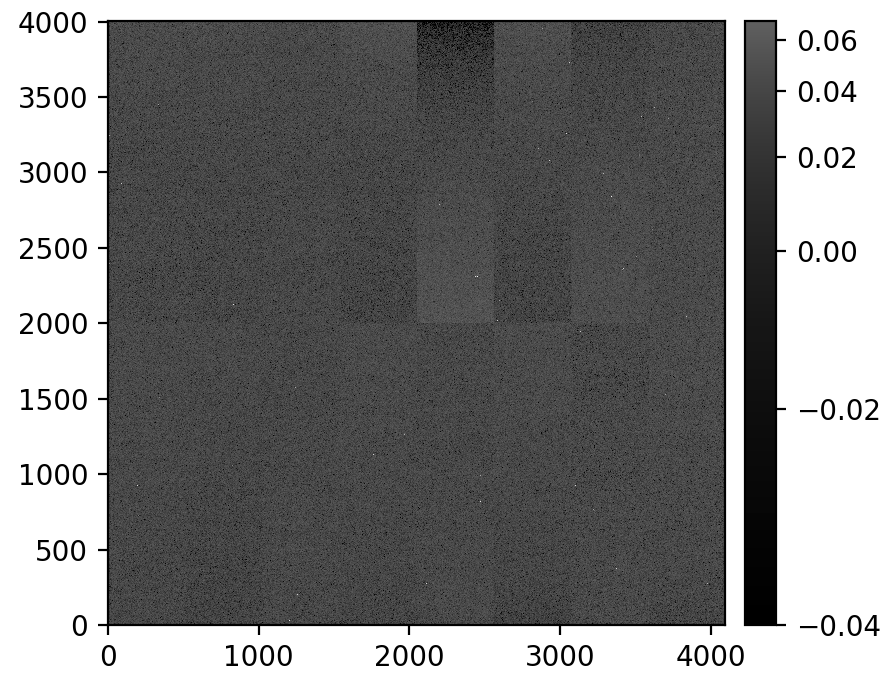
\includegraphics[width=\textwidth]{Figures/Super_dark_55.png}
     \end{subfigure}
     \hfill
     \begin{subfigure}[b]{0.49\textwidth}
         \centering
         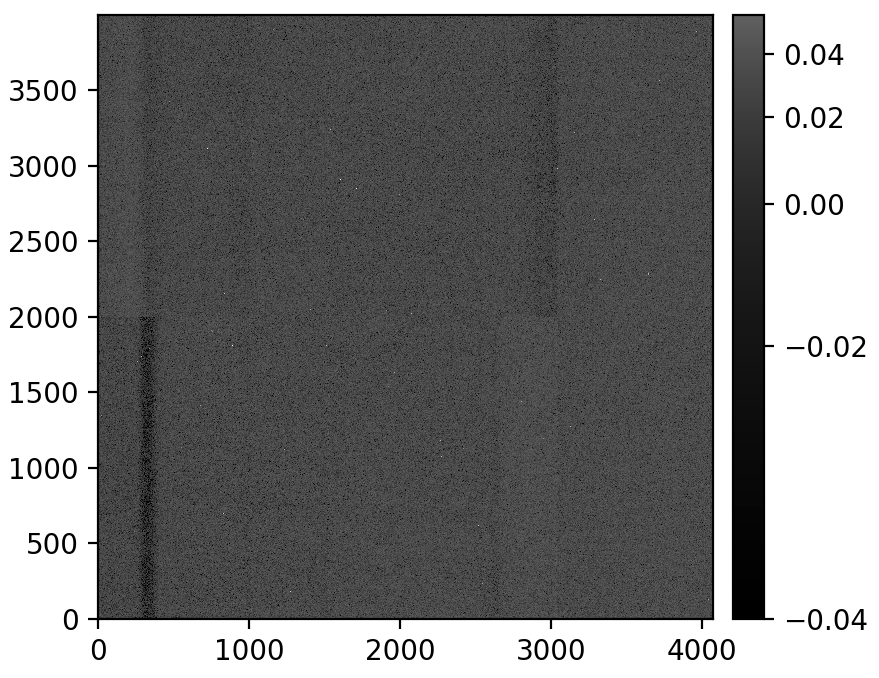
\includegraphics[width=\textwidth]{Figures/Super_dark_74.png}
     \end{subfigure}
        \caption{Masterdarks images for detectors 55 (E2V) on the left and 74 (ITL) on the right}
        \label{fig:superdark}
\end{figure}


\subsection{Photon Transfer Curve (PTC)}
The PTCs were generated for the entire LSSTCam focal plane using the \textit{DM stack}\footnote{The PTCs are constructed with the code available in the repository \href{https://github.com/lsst/cp_pipe}{cp\_pipe}}, which allows estimating the gain, read noise, $a_{00}$ (parameter related to the BF effect), and turnoff (associated with the FWC) from a fit to the shape of the PTC. This code implements equations 16 and 20 of the \cite{2019A&A...629A..36A} article: equation 16 corresponds to the exponential approximation (EXPAPPROXIMATION), which uses only the variance ($C_{00}$); while equation 20 is the full model (FULLCOVARIANCE), and implements the covariance matrix. In this work, we used EXPAPPROXIMATION, which is described by the following equation:

\begin{equation}
    C_{00} = \frac{1}{2 g^2 a_{00}} [\exp (2 a_{00} \mu g) - 1] + \frac{n_{00}}{g^2}
    \label{eq:Astier16}
\end{equation}

where $C_{00}$ is the variance, $g$ is the gain, $a_{00}$ is always negative and is related to the B-F effect, $mu$ is the mean, and $n_{00}$ ($el^{2}$) is the noise. According to \cite{2019A&A...629A..36A}, a negative value of $a_{00}$ leads to the variance of a flat field not growing as fast as the mean does. In the case where there is no BF effect, i.e., each pixel is independent of the other and is described by a Poisson statistic, the mean, gain, and variance are directly related through the equation:

\begin{equation}
    V = \frac{\mu}{g}
    \label{eq:gain_Poisson}
\end{equation}

where $V$ is the variance of a flat field, $\mu$ is the mean, and $g$ is the gain.



\subsection{Gain from flat pairs} \label{subsec:method_gainflat}
An independent method for calculating a sensor's gain is using flat field pairs with equal exposure times. Since each CCD is composed of 16 segments, each with its amplifier, a gain value is obtained for each segment. For this purpose, LSST has the function \href{https://github.com/lsst/cp_pipe/blob/main/python/lsst/cp/pipe/ptc/cpExtractPtcTask.py#L679}{Gain from flat pairs}, which was analyzed in detail in this work.

\vspace{3mm}
We aim to quantify the difference between the gain calculated from the fit to the PTC and this independent method using flat field pairs with equal exposure times. For this, we initially calculate the average flux in ADU with each flat pair, the read noise, and the gain. The latter is estimated employing the equation of \cite{2014JInst...9C4023L}:

\begin{equation}
    \frac{1}{g} = \Big \langle \frac{(I_1 - I_2)^2}{I_1 + I_2} \Big \rangle 
    \label{eq:Lupton}
\end{equation}

where $g$ is the gain, $I_1$ is the first flat image, and $I_2$ is the second flat image, both taken at the same exposure time. The expected value over all pixels is the inverse of the gain. Considering corrections for read-out noise, the equation takes the following quadratic form:

\begin{equation}
    \frac{1}{g} = \Big \langle \frac{(I_1 - I_2)^2}{I_1 + I_2} \Big \rangle - \frac{1}{\mu} (N^2-\frac{1}{2} g^2)
    \label{eq:gain_corrected}
\end{equation}

Where $\mu = 0.5(\mu_1 + \mu_2)$, with $\mu_1$ and $\mu_2$ being the average values for each of the flat images, and $N$ is the read-out noise. The equation above has three variants: NONE, SIMPLE, and FULL, with NONE being equivalent to Equation \ref{eq:Lupton}. The remaining two cases are as follows:

\begin{align}
g = \begin{cases}
  \frac{1}{K - \frac{1}{\mu}(N^2 - \frac{1}{2} g^2)} & \mbox{SIMPLE} \\
  \frac{\mu + \sqrt{\mu^2 - 2 \mu K + 2 N^2}}{2 K \mu - 2 K^2} & \mbox{FULL}
\end{cases}
\label{eq:sol_gain_corrected}
\end{align}

where $K$ is equal to Equation \ref{eq:Lupton}. In the SIMPLE case, $g = 1/K$, while in the FULL case, the quadratic equation is solved, and the result is taken to have physical meaning. Once we have the gains calculated from pairs of flats for flows between 0 and $\sim 10000$ ADU, we calculate the relative percentage error with the gain obtained from the fit to the PTC using Equation \ref{eq:sol_gain_corrected} with the FULL type correction:

\begin{equation}
    \mbox{Relative\_error} [\%] = \frac{|gain_{PTC} - gain_{flats}|}{gain_{PTC}} \times 100 \% 
    \label{eq:error_relativo_gain}
\end{equation}

Subsequently, a linear low-flow fit was performed, which we considered to be between 5000 and 10000 ADU. The low-flow fit has the following form:

\begin{equation}
    \mbox{Relative\_error}_{LF} [\%] = m F + \mbox{offset}
\end{equation}

Where $m$ is the slope of the fit, $F$ is the flux, and \textit{offset} is the intercept with the $y$-axis. These parameters are used to quantify the error variation in the specified flow range and the base error between the PTC gain and that calculated with the flats. We generated histograms of these parameters to examine the behavior of the vendor's data and extract general trends. To exclude outliers, i.e., CCD segments with abnormal behavior, we utilized the \textit{sigma\_clip} and \textit{sigma\_clipped\_stats} functions from \cite{2018AJ....156..123A}. These functions allowed us to cut the data such that only values within $3 \sigma$ of the median were retained, and we performed this operation iteratively three times to ensure robustness.


 \begin{figure}[!htb]
     \centering
     \begin{subfigure}[b]{\textwidth}
         \centering
         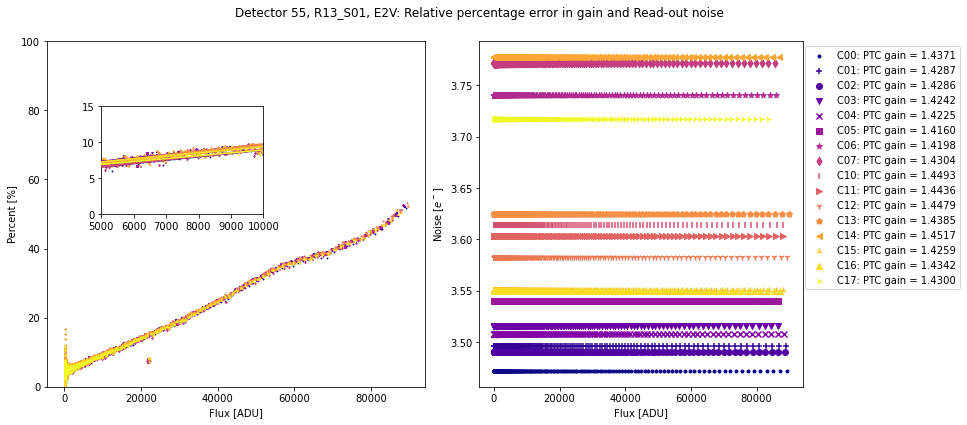
\includegraphics[width=\textwidth]{Figures/Relative_Error_Gain_Noise_detectorR13_S01_old.png}
     \end{subfigure}
     \vspace{3mm}
     \begin{subfigure}[b]{\textwidth}
         \centering
         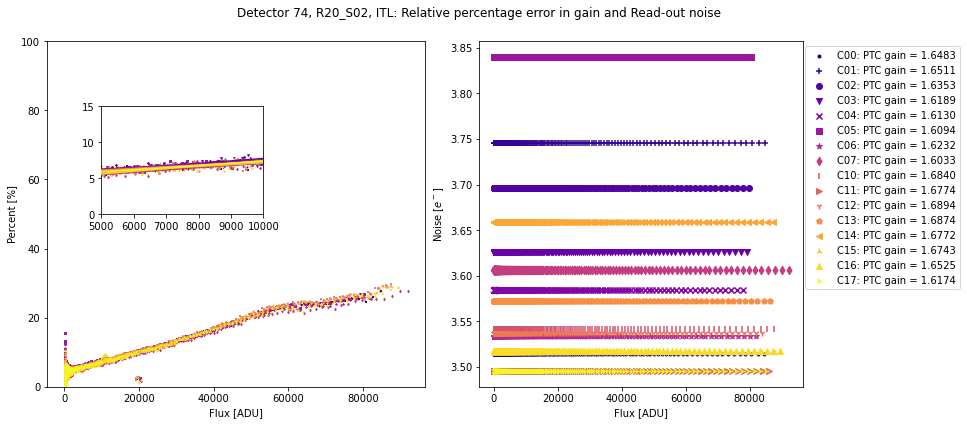
\includegraphics[width=\textwidth]{Figures/Relative_Error_Gain_Noise_detectorR20_S02_old.png}
     \end{subfigure}
        \caption{The relative percentage error between the gain estimated by the PTC and the gain calculated from two flat images is shown in the left panels, while the read-out noise of each amplifier is shown in the right panels. The upper panel displays the results for detector 55 (R13\_S01) with vendor E2V, and the lower panel shows the results for detector 74 (R20\_S02) from vendor ITL. Each color and symbol in the plots represents the relative percentage error for one of the 16 segments that make up each CCD. The embedded image in the left panels shows the percentage error specifically between 5000 and 10000 ADU, corresponding to the low flux regime where a linear fit is performed. The data used to construct these plots includes only values below the PTC turnoff.}
        \label{fig:relative_error_oldcode}
\end{figure}


\begin{figure}[!htb]
    \centering
    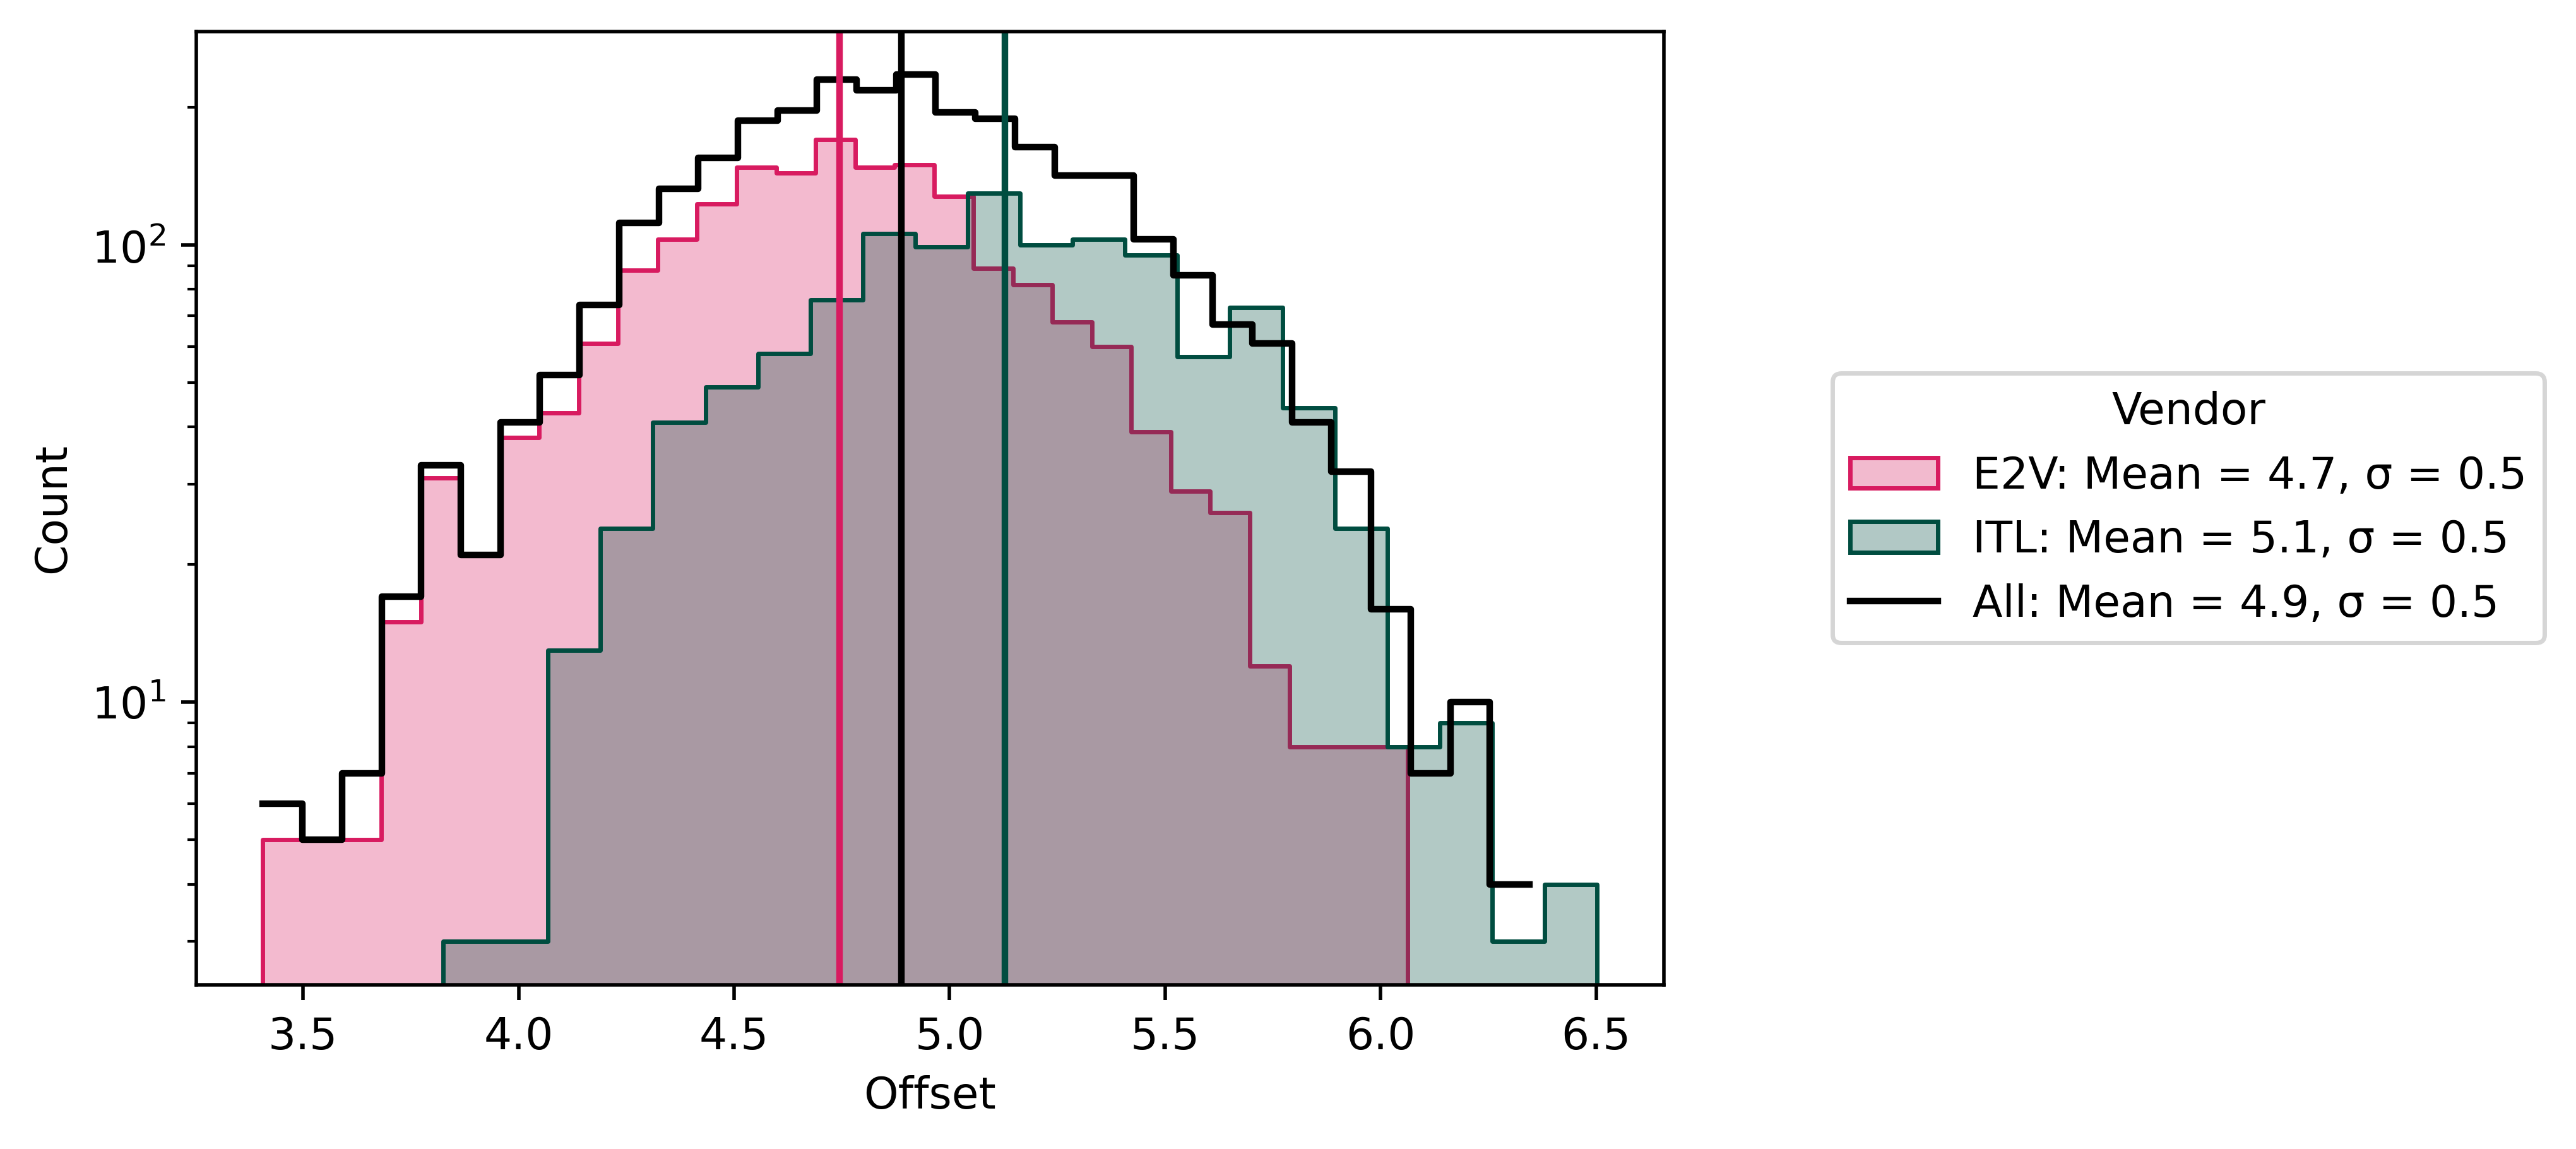
\includegraphics[width=\textwidth]{Figures/Histogram_offset_old.png}
    \caption{The histograms display the offset value obtained from the linear fit for flows between 5000 and 10000 ADU, representing the relative percentage error between gains. The magenta distribution represents the results for vendor E2V, with a mean of $(4.7 \pm 0.5)$ \%. The blue distribution shows the results for vendor ITL, with a mean of $(5.1 \pm 0.5)$ \%. The black distribution represents the histogram of all data without discrimination by vendor, with a mean of $(4.9 \pm 0.5)$ \%. Vertical lines indicate the value of the mean for each distribution.}
    \label{fig:hist_offset_old}
\end{figure}

\subsubsection{Simulation} \label{subsubsec:method_Simulation_Gain}

The methodology outlined in Section \ref{subsec:method_gainflat} and the utilization of LSST software version \textit{w\_2022\_27} yielded the results depicted in Figures \ref{fig:relative_error_oldcode} and \ref{fig:hist_offset_old}. Figure \ref{fig:relative_error_oldcode} showcases the relative percent error between the gains for E2V sensor 55 (top panel) and ITL sensor 74 (bottom panel) over the flow range below the PTC turnoff. The embedded plot on the left displays the behavior between 5000 and 10000 ADU, along with the corresponding linear fit, while the plot on the right shows the error for each CCD segment within the same flow range. Notably, the embedded plot reveals that the relative error has an offset exceeding 5\% for these two sensors, prompting us to construct a histogram with the offset values for the entire focal plane to determine if this behavior is widespread. Figure \ref{fig:hist_offset_old} confirms that this relative error is a prevalent characteristic exhibited by all sensors, with an average base error of $\sim 5$\%, which we consider relatively high. Thus, we further investigated this issue through simulations.

\vspace{3mm}

Various factors, including potential overestimation of the read-out noise, the influence of masks used in the images, or assumptions about the distribution for the operations between flat images as given by Equation \ref{eq:ratioIm}, could contribute to the observed behavior. The \textit{w\_2022\_27} version of the \textit{DM stack} assumes that Equation \ref{eq:ratioIm} follows a Gaussian distribution.

\begin{equation}
      \frac{(I_1 - I_2)^2}{I_1 + I_2} 
      \label{eq:ratioIm}
\end{equation}

To better understand and address this issue, further analysis and simulations were conducted. If the distribution is found to deviate from a Gaussian distribution, the distribution statistics would need to be modified accordingly. To explore possible variables, we conducted simulations in three different cases, as described below:


\begin{itemize}
    \item \textbf{Case 1 - Noise Overestimation}: Two data sets were constructed following a Poisson distribution for the flow, with an expected value ranging from 5000 to 10000 ADU. In our case, we chose 5000 ADU as the expected value. The Poisson distribution is given by:
 
    \begin{equation}
        f(k;\lambda) = \frac{\lambda^k e^{-\lambda}}{k!} \implies f(k;5000) = \frac{5000^k e^{-5000}}{k!}
    \end{equation}
    \label{eq:dist_Poisson}

    where $\lambda$ is the expected value and $k$ is the number of events. To this data, we added Gaussian noise with a mean of zero and a dispersion value that we assume as the read-out noise, given by:
    
    \begin{equation}
        p(x) = \frac{1}{\sqrt{2 \pi \sigma^2}} \exp \Big(-\frac{(x - \mu)^2}{2\sigma^2} \Big) \implies p(x) = \frac{1}{\sqrt{2 \pi N^2}} \exp \Big(-\frac{x^2}{2N^2} \Big)
        \label{eq:gaussian_noise}
    \end{equation}
    
    where $\mu$ is the mean, $\sigma$ is the standard deviation, and $N$ is the read-out noise that we assume. Finally, we apply the methodology described in Section \ref{subsec:method_gainflat} for all types of gain correction: NONE, SIMPLE, and FULL, and calculate the relative error using a base gain (chosen as 2.0) to verify if we can replicate the observations in Figure \ref{fig:relative_error_oldcode}, specifically a base error above 5\%.

    \item \textbf{Case 2 - Pixel Masks}: In this step, pixel masks are added to Case 1. The respective mask is extracted from each flat image, where each flat has an average of 5000 ADU counts. This mask filters out suspicious, bad, dead, and saturated pixels. Next, a Poisson distribution is generated with the dimensions of one of the CCD segments for which the masks were extracted, i.e., $size_x = 2002$ and $size_y = 512$, along with its respective Gaussian noise. The generated mask is then applied to each array using the \textit{Numpy} function \citep{2020Natur.585..357H} \textit{ma.masked\_where}.

    
    \begin{figure}[!htb]
        \centering
        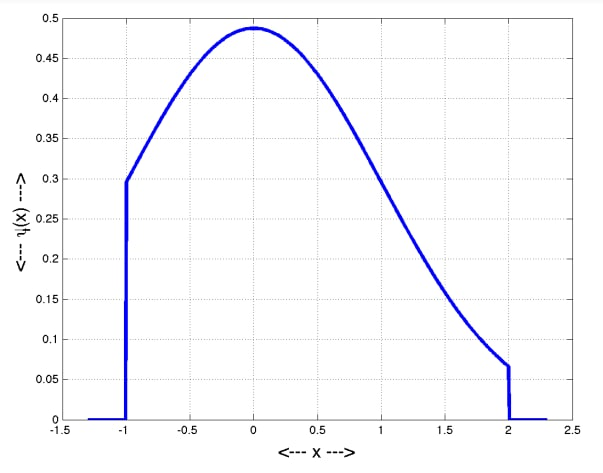
\includegraphics[width=0.5\textwidth]{Figures/Truncated_Gaussian.jpg}
        \caption{The truncated Gaussian distribution with a zero mean and standard deviation is represented by $\psi(0,1,a = -1, b = +2; x)$. This figure is sourced from \cite{burkardt2014truncated}.}
        \label{fig:truncated_gaussian_dist}
    \end{figure}

    \textbf{Case 3 - Statistics control}: Building upon Case 2, we incorporate statistics control by assuming that the distribution of equation \ref{eq:ratioIm} follows a Gaussian distribution. Similar to the approach used in section \ref{subsec:method_gainflat}, we truncate the distribution by keeping only the data points that fall within $5.5 \sigma$ of the mean, and we repeat this process for three iterations. When the distribution of equation \ref{eq:ratioIm} is Gaussian, the mean of the symmetrical truncated distribution is the same as the original one, and the mean of non-symmetrical truncated distribution can be calculated as:
    
    \begin{equation}
        \mu = \overline{\mu} - \overline{\sigma} \frac{\phi (0,1; \beta) - \phi (0,1; \alpha)}{\Phi (0,1; \beta) - \Phi (0,1; \alpha)} \; \; \; ; \alpha = \frac{a-\overline{\mu}}{\overline{\sigma}} , \beta = \frac{b -\overline{\mu}}{\overline{\sigma}}
        \label{eq:truncated_dist}
    \end{equation}

    where $\alpha$ and $\beta$ are standardized variables, $a$ and $b$ are the cutoff values for the lower and upper tails of the distribution, respectively, $\overline{\mu}$ and $\overline{\sigma}$ are the statistics of the original distribution, $\phi$ represents the normal probability density function (PDF), and $\Phi$ represents the Normal cumulative distribution function (CDF). Figure \ref{fig:truncated_gaussian_dist} illustrates this case for $a=-1$ and $b=+2$. However, when the distribution is symmetrically truncated, i.e., $-a=b$, the numerator of the second term in the above equation becomes zero, and the mean of the truncated and original distribution is simply:
    
    \begin{equation}
        \mu = \overline{\mu}
        \label{eq:truncated_dist_simetric}
    \end{equation}

    This implies that the mean of the truncated and original distribution are equal, as mentioned earlier. We use this result to calculate the expected value of equation \ref{eq:Lupton} in order to determine the gain solutions for the NONE, SIMPLE, and FULL corrections. As an additional step, we examine the shape of the distribution of equation\ref{eq:ratioIm}; if the distribution of equation \ref{eq:ratioIm} is not Gaussian, no truncation is applied, and the expected value of equation \ref{eq:Lupton} is calculated using the arithmetic mean.

\end{itemize}


\subsection{No linearity Correction} \label{subsec:method_Linearity}

To study the impact of linearity correction on the PTC shape and parameters, we applied a 12-node spline linearizer to detectors 32 (ITL) and 139 (E2V). The effectiveness of this method was established in \citeds{RTN-055}, where it was found that a 12-node spline significantly corrects the nonlinearity effect and reduces residual dispersion. All configurations remained unchanged, except for the linearity correction (see table \ref{tab:config_linearity}).


\begin{table}[!htb]
\centering
\caption{The configuration used to generate the PTCs when we include the linearity correction (the parameter 'doLinearize' is set to 'true').}
\label{tab:config_linearity}
\resizebox{\textwidth}{!}{%
\begin{tabular}{cccc}
\hline
\multicolumn{4}{c}{\textbf{Configurations}} \\
\hline
\hline
  doWrite: true       &  doLinearize: true      &  doFlat: false       &  doInterpolate: false  \\
  doOverscan: true    &  doCrosstalk: false      &  doFringe: false     &  doSaturation: false   \\
  doAssembleCcd: true &  doBrighterFatter: false &  doApplyGains: false &  doSaturationInterpolation: false  \\
  doBias: true        &  doDark: true            &  doDefect: true      &  growSaturationFootprintSize: 0 \\
  doVariance: true    &  doStrayLight: false     &  doNanMasking: true  &  ptcFitType: EXPAPPROXIMATION \\
  \hline
\end{tabular}%
}
\end{table}

Subsequently, plots of the ratio of Variance to Mean vs Mean are constructed, normalizing the variance. This allows for analysis of whether the bump between 50000 and 60000 ADU is corrected. Additionally, a relative percentage error between the parameters obtained from the PTC fit with and without linearity correction is calculated to quantify the effect on these parameters. Finally, a comparison is made to check if the parameters and/or the shape of the PTC changed compared to the version without correction for nonlinearity.


\subsection{Crosstalk Correction} \label{subsec:method_Crosstalk}

The LSSTCam's full focal plane can be read out in 2 seconds, and the combination of high-speed, high-resistivity silicon components and close spacing between each channel makes it more susceptible to electronic crosstalk compared to other mosaic cameras \citep{2015JInst..10C5010O}.

\vspace{3mm}

\begin{figure}[!htb]
    \centering
    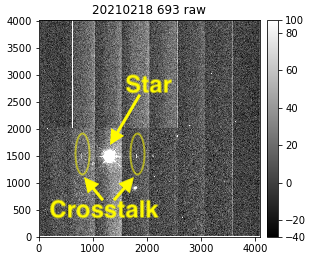
\includegraphics{Figures/Crosstalk_effect.png}
    \caption{An image of a bright star captured with the 1.2m auxiliary telescope at the Vera Rubin Observatory, revealing crosstalk in segments adjacent to the star's image.}
    \label{fig:crosstalk}
\end{figure}

Electronic crosstalk occurs in CCDs with multiple channels that are read simultaneously and coupled, resulting in ghost images generated in adjacent segments when a bright source is detected in a channel due to this coupling \citep{2020SPIE11454E..39S}. This effect is illustrated in Figure \ref{fig:crosstalk}, where ghost signals are observed in the lateral segments of the detector. Figure \ref{fig:crosstalk_matrix} shows a heat map on the left for ITL detector 32 and on the right for ITL detector 139, depicting the crosstalk coefficients in blue colors, with the observation that the crosstalk pattern differs per vendor. These coefficients are incorporated into a configuration file in the LSST software to regenerate the PTC with this correction.

Finally, similar to the approach in Section \ref{subsec:method_Linearity}, a comparison was made to check whether the parameters and/or the shape of the PTC changed compared to the version without correction for crosstalk.


\begin{figure}[!htb]
     \centering
     \begin{subfigure}[b]{0.49\textwidth}
         \centering
         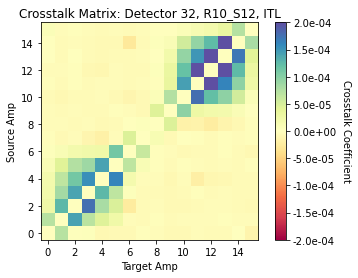
\includegraphics[width=\textwidth]{Figures/Crosstalk_32.png}
     \end{subfigure}
     \hfill
     \begin{subfigure}[b]{0.49\textwidth}
         \centering
         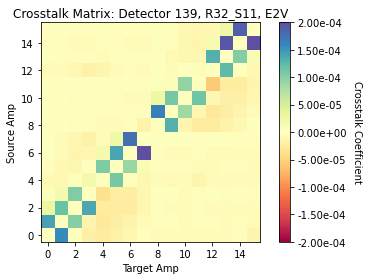
\includegraphics[width=\textwidth]{Figures/Crosstalk_139.png}
     \end{subfigure}
        \caption{Crosstalk matrix shown on the left for detector 32 (ITL) and on the right for detector 139 (E2V).}
        \label{fig:crosstalk_matrix}
\end{figure}